\documentclass[fleqn]{jbook}
\usepackage{physpub}

\begin{document}

\begin{question}{教育 英語}{}

\begin{subquestions}
\SubQuestion
  以下の文章を読み、下線部(1)〜(6)を和訳せよ。
\baselineskip=12pt

   \underlineeng{(1)A scientific model begins with a real physical
  object or system, replaces the original object with a simpler object,
  and then represents the simplified object with equations describing
  its behavior.}
  \underlineeng{(2)Like a toy boat, a scientific model is a
  scaled-down version of a physical system, missing some parts of the
  original.}
  \underlineeng{(3)Deciding what parts should be left out requires
  judgement and skill.}
  \underlineeng{(4)The omission of essential features makes the
  model worthless.}
  \underlineeng{(5)On the other hand, if nothing is left out, no
  simplification has been made.}
  In making a model of a swinging pendulum, for example, we might at
  first try to include the detailed shape of the weight at the end,
  the density and pressure of the air in the room, and so on. Finding
  such a description too complex to manage, we could replace the
  weight by a round ball neglect the air completely. This much simpler
  system, in fact, behaves almost exactly like the original. If, on
  the other hand, we left out gravity, the resulting theoretical
  pendulum would not swing back and forth.
  \underlineeng{(6)By solving the equations of a model,
  predictions can be made about the original physical system and then
  tested.}

  \rightline{--- quoted from `Origin' by A. Lightman and R. Brawer}
\baselineskip=15pt

\SubQuestion
  以下の各文章は,$P$と$I$との関係に関するある実験結果について説明した
  ものである。各文を英訳せよ。解答では、$P$,$I$はそのままでよい。
%
  \begin{subsubquestions}%
  \SubSubQuestion
    これまでの研究において我々は、$P$は温度に依存しないと仮定して、
    ある特定の温度で$I$の関数として$P$を測定していた。
  \SubSubQuestion
    この仮定の妥当性を検討するために本実験では、様々な温度で$P$を
    測定した。
  \SubSubQuestion
    図1で、黒丸(filled circles)は$25\degC$、黒三角(filled triangles)は
    $20\degC$、白ヌキの四角(open squares)は$15\degC$における測定結果を
    示す。\\
  \parbox[t]{80mm}{
  \SubSubQuestion
    $ 25\degC $において、$I$が$300\mu\Unit{mol\,m^{-2}s^{-1}}$以下では $I$の増加に伴って$P$は直線的に増加し、$300\Unit{\mu mol\,m^{-2}s^{-1}}$以上では一定の値$0.4\Unit{\mu mol\,O_2 mg^{-1}h^{-1}}$となる。
  \SubSubQuestion
    $P$の一定値は、$15\degC$では$25\degC$の4分の1である。
  \SubSubQuestion
    $P$が一定の値に達するときの$I$の値は温度の低下に伴って小さくなる。
  \SubSubQuestion
    一方、$I$が0の時の$P$の値は、温度が高いほど小さい。
  \SubSubQuestion
    こうした結果は、$P$が温度に依存しないという仮定に反する。
  \SubSubQuestion
    より高温での$P$と$I$との関係について、今後さらに実験が必要である。
  }\parbox[t]{80mm}{
  \begin{center}
    \mbox{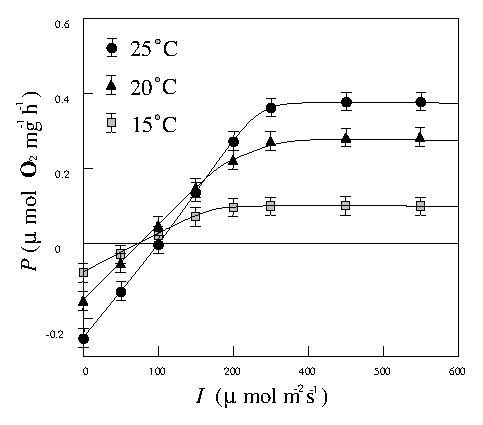
\includegraphics[clip]{1995engl-1.eps}}
  \end{center}}
  \end{subsubquestions}

\newpage
\SubQuestion

  以下の文章を読み、文中の内容に沿って、設問に日本語で答えなさい。
  各設問への解答の内容は、互いに重複する部分があっても良い。
\baselineskip=12pt

   One way of generating ideas is just to generate them---that is,
  to talk out or write down what ever comes into your head about the
  topic you want to write about. Don't worry about whether the ideas
  are good or adequate or complete; just get them down. The purpose
  of brainstorming is to provide yourself with some notes that you
  can use to further stimulate your thinking and organizing. If you
  feel intimidated by a blank page, you might try talking into a tape
  recorder about your topic and then listening to what you've said
  and writing down the good ideas that are there.

   Brainstorming is a very intuitive process. You just follow your
  ideas wherever they lead and take notes to record your mental
  journey. It's important that you not censor an idea before it has a
  chance to flower, but just generate it. Evaluation and organization
  of the ideas will come later, but you can't evaluate or organize
  something that isn't there.

   Brainstorming is often best done in collaboration with other
  people. By ``bouncing ideas'' off of others, you can stimulate their
  thinking and get them to produce ideas of their own. As with any
  kind of brainstorming, the important thing is not to evaluate or
  criticize ideas but just to generate them.

   If you are collaborating with others who are not always in your
  room or building, you might see if you and your collaborators can
  collaborate via computer. To do this you will all need access to
  computers on a network with connects each computer.
%
  \begin{flushright}
  ---from ``Technical Writing and Professional Communication%
     For Nonnative Speakers of English'',\\
     2nd edition, by T.N.Huckin and L.A.Olsen
  \end{flushright}
%
\begin{list}{}{\itemindent=0mm \labelwidth=28mm \leftmargin=28mm
\topsep=0mm \itemsep=0mm \parsep=0mm}
\item[intimidate:(verb)\hfill]
frighten somebody (in order to make him do something);
{\it intimidate a witness into silence}, e.g. by threating him.

\item[intuitive:(adj.)\hfill]
(1) of or coming from intuition;
{\it intuitive feeling}\\
(2)possessing intuition;
{\it Are women more intuitive than men?}

\item[intuition:(noun)\hfill]
(1) (power of)understanding things immediately, without the need for
conscious reasoning or study.
{\it Intuition told me you were here.}\\
(2) piece of knowledge gained by this power.
{\it I had a sudden intuition about the missing jewels.}

\item[censor:(verb)\hfill]
examine or remove parts from something;
{\it the censored version of a film.}

\item[censor:(noun)\hfill]
person authorized to examine books, films, plays, letters etc.
and remove parts which are considered indecent, offensive,
politically unacceptable or (esp. in  war) a threat to security.
\end{list}

\rightline{---According to Oxford Advanced Lerner's Dictionary with modification.}

\baselineskip=15pt
  \begin{subsubquestions}
  \SubSubQuestion
    ブレインストーミングとは何か、4つのポイントを挙げて、全体で5行以内
    で述べなさい。

  \SubSubQuestion
    ブレインストーミングを実行する方法を、4つのポイントを挙げて、全体で
    5行以内で述べなさい。

  \SubSubQuestion
    ブレインストーミングを行う際に避けるべきことを、3つのポイントを
    挙げて述べ、それは何故かを2つのポイントを挙げて述べ、全体で5行以内
    でまとめなさい。
  \SubSubQuestion
    同僚とともにブレインストーミングすると良いのは何故か、5行以内で
    述べ、答案の中で、``bouncing''の意味を最も捉えたと貴方が考えている
    箇所には、一カ所だけ下線を引きなさい。

  \end{subsubquestions}


\end{subquestions}
\end{question}
\begin{answer}{教育 英語}{}
\begin{subanswers}
\SubAnswer

  {\bf 全訳}

  \underlinejpn{(1)科学のモデルは、実在する物体や系から始まり、元々の物体をより簡単な物体に置き換え、そしてその簡単化された物体の振る舞いを記述する数式によって、その物体を表現する}。
  \underlinejpn{(2)おもちゃの船のように、科学のモデルは物理系を縮小した物であり原型の一部を省いている}。
  \underlinejpn{(3)どこを残すのかを決めるには判断力と技が必要である}。
  \underlinejpn{(4)基本的な特徴を省いてしまっては、モデルは無意味な物となる}。
  \underlinejpn{(5)逆に、何も省かないと、なんら簡単化されない}。
  例えば、振れている振り子のモデルを作るとき、まず初めは、終端にある
  重りの細かい形、部屋の空気の密度と圧力、等々を考慮に入れようとする
  だろう。そのような記述が、実現するには複雑すぎると気づき、重りを
  球形のボールに置き換え、空気を完全に無視できよう。この、より簡単な
  系は、実際には、元の系とほとんど寸分違わぬ振る舞いをする。一方で、
  もし重力を省いていたら、その結果の理論的振り子は前後に振れることは
  なかっただろう。
  \underlinejpn{(6)モデルの数式を解くことによって、原型となる物理系の予測ができ、そして検証することができる}。


\SubAnswer
\baselineskip=12pt
  \begin{subsubanswers}
  \SubSubAnswer
    In our previous researches, we assumed no dependence of $P$ on 
    temperature. For that reason, we measured $P$ as a function of
    $I$ at the consistent temperature. 
  \SubSubAnswer
    To verify this assumption, we measured $P$ at various temperatures.
  \SubSubAnswer
    In fig.1, measurement results for various temperatures are shown
    as, filled circle for $25\degC$, filled triangles for $20\degC$,
    open squares for $15\degC$.
  \SubSubAnswer
    At $25\degC$, $P$ rises linearly as $I$ rises when $I$ is bellow
    $300\mu\Unit{mol\, m^{-2} s^{-1}}$, and $P$ is constant and at 
    $0.4\mu\Unit{mol\, O_2 mg^{-1} h^{-1}}$ when $I$ is over 
    $300\mu\Unit{mol\, m^{-2} s^{-1}}$.
  \SubSubAnswer
    The constancy of P at $15\degC$ is one fourth of that at $25\degC$.
  \SubSubAnswer
    The value of $I$ when $P$ becomes constant drops as temperature
    drops.
  \SubSubAnswer
    On the other hand, $P$ for $I=0$ gets smaller for higher
    temperatures.
  \SubSubAnswer
    These results are contrary to the assumption of no dependence of
    $P$ on temperature. 
  \SubSubAnswer
    More experiments are required to investigate the relation between
    $P$ and $I$ for higher temperature.
  \end{subsubanswers}

\baselineskip=15pt
\SubAnswer

  \begin{subsubanswers}
  \SubSubAnswer
    何かの主題について、(1)直感的に思いつくことを、(2)その考えに
    ついて善し悪しの判断を先送りして、(3)記録に残し、後でそれを参照
    して、(4)自分の考えを発展させること。
  \SubSubAnswer
    (1)決められた主題について、(2)思い浮かぶことを、(3)善し悪しの判断
    をせずに、(4)書いたり録音したりする、という方法。
  \SubSubAnswer
    避けるべき事は、ブレーンストーミングの(1)実行中に、(2)記録すべきか
    迷ったり、(3)評価したり、まとめたりすることである。\\
    なぜなら、記録しなければ考えが大きく(1)発展していく可能性を潰して
    しまうし、記録が十分に無ければ(2)判断やまとめの材料が得られないから。
  \SubSubAnswer
    相手に投げかけた自分の思いつきが、相手の新たな発想を促し、相手
    の新たな思いつきが、自分の発想を刺激して、
    \underline{発想を投げかけ合う}ことによって、一人では限界がある
    発想を広げることが出来るから。
  \end{subsubanswers}

  {\bf 全訳}

   アイディアを生み出す一つの方法は、ひたすら生み出すことに徹すること
  だ。それはつまり、あなたが書きたいと思う主題について、頭に思い浮か
  ぶままに口に出すか、書き下すのだ。アイディアが良いか、適切か、完全
  かなどは気にする必要はない。とにかく書き下すのだ。ブレーンストーミ
  ングの目的は思考をより活発化させる注釈を得ることである。もし、空白
  のページに恐れをなしたら、テープレコーダにあなたの主題について吹き
  込み、後でそれを聞いて、紙に良い考えを書けばよいのだ。

   ブレーンストーミングは、とても直感的なものである。考えの赴くままに
  従って、精神の旅の記録として、ノートをとるのだ。浮かんだアイディア
  が花開く前に、吟味せずに、ただ生み出すことが重要である。評価とまと
  め上げも、先立つアイディアがなければ出来ないのだ。

   ブレーンストーミングは、大抵の場合、他の人と共同ですることによっ
  て、もっと上手く行く。他の人と、「アイディアを弾ませ」合うことで、
  相手の考えを刺激し、アイディアを生み出させて上げることが出来る。ど
  のブレーンストーミングでも言えることだが、重要なことは、アイディア
  を評価したり、批判したりせず生み出すことに専念することだ。

   もし、同じ部屋や同じ建物にいない人と、共同作業しているなら、相手が
  コンピュータで協力しあえるか調べてみると良い。これには、共同作業者が
  皆、互いを結ぶネットワーク上のコンピュータを使えることが必要である。

\end{subanswers}
\end{answer}


\end{document}
